\documentclass[a4paper, 12pt]{extarticle}
\usepackage[dvipsnames]{xcolor}
\usepackage[top=70pt,bottom=70pt,left=48pt,right=46pt]{geometry}
\definecolor{header}{RGB}{92,184,92}
\definecolor{defenition}{RGB}{217,83,79}
\definecolor{main_title}{RGB}{66,139,202}
\definecolor{sub_header}{RGB}{91,192,222}
\usepackage[english, russian]{babel}
\usepackage[utf8]{inputenc}
\usepackage{amsmath}
\usepackage{svg}
\usepackage{listings}
\usepackage{graphicx}
\usepackage{amsmath}
\title{\textcolor{main_title}{Диод в качестве контролируемой напряжением ёмкости}}
\author{Шмаков Владимир Евгеньевич - ФФКЭ гр. Б04-105}






\begin{document}
\maketitle

\section*{\textcolor{header}{Цель работы}}
\begin{itemize}
    \item Разработать методику измерения зависимости ёмкости полупроводникого диода от величины обратного напряжения.
    \item Измерить зависимость ёмкости от напряжения.
\end{itemize}


\section*{\textcolor{header}{Теоретические сведения}}

\begin{minipage}{0.6 \textwidth}
    \includegraphics*[width = \linewidth]{pics/isolator.jpg}
\end{minipage}
\hfil
\begin{minipage}{0.4\textwidth}\raggedright
    \textcolor{defenition}{Полупроводник} — материал, занимающий промежуточное место между изоляторами и проводниками. 
    При нулевой температуре, зона проводимости полупроводника оказывается пустой(это «роднит» полупроводники и изоляторы).
    Однако расстояние между валентной зоной и зоной проводимости у полупроводника значительно меньше чем у изолятора(смотрите рисунок слева).
\end{minipage}
\noindent 
\\
Введение в полупроводник примесей приводит к появлению разрешенных уровней в запрещенной зоне. 
Примеси, которые приводят к образованию в полупроводнике уровней вблизи нижнего края зоны проводимости называются \textcolor{defenition}{донорными}.
Примеси, приводящие к появлению уровней вблизи границы валентной зоны называются \textcolor{defenition}{акцепторными}. Если концентрация акцепторов 
в полупроводнике превышает концентрацию доноров, 
то говорят что полупроводник является проводником \textcolor{defenition}{p - типа}. 
В противном случае, говорят что полупроводник является проводником \textcolor{defenition}{n - типа}.


Соединим проводник $p$-типа с полупроводником $n$-типа. Из полупроводника 
$n$ - типа электроны устремятся в область $p$ - типа. Дырки, в свою очередь,
устремтся из области $p$-типа в область $n$ - типа. При возникновениии равновесия
уровни Ферми контактирующих полупроводников сравняются, а в месте контакта
возникнет обеднённая область(смотрите рисунок $\ref{fig:ravnovesie}$).

\begin{figure}[htbp]
    \centering
    \includegraphics*[width = 0.5 \textwidth]{pics/ravnovesie.png}
    \caption{Обеднённая зона в месте контакта(сверху). Распределение электрического поля(снизу).
    Поле направлено из n-области в p-область.}
    \label{fig:ravnovesie}
\end{figure}

Такой $pn$ переход может рассматриваться как конденсатор. Обкладками конденсатора служат границы
области обеднения. Зона обеднения выступает в качестве диэлектрика. На обкладках содержатся носители
зарядя - электроны и дырки.

При приложении обратного напряжения, ширина обеднённой зоны увеличивается,
что приводит к уменьшению ёмкости рассматриваемого конденсатора.

Зависимость ёмкости от напряжения выражается формулой $\ref{capacity_by_volt}$.
$ m$ принимает значения от $1 / 2$ до $1 / 3$.
$V_0$,$ K$ - постоянные, зависящие от степени легирования полупроводников.
\begin{equation}
    C = \frac{K}{(V_0 - V)^m}
    \label{capacity_by_volt}
\end{equation}

\section*{\textcolor{header}{Методика}}
\subsection*{\textcolor{sub_header}{Оборудование}}
\begin{itemize}
    \item Катушка 
    \item Набор ёмкостей
    \item Полупроводниковый диод
    \item Диод Шоттки
    \item Набор резисторов
    \item Операционный усилитель TL072
    \item Две девятивольтовые батарейки
    \item Аудиокарта 
    \item Интерпретатор Python и библиотеки scipy, numpy, matplotlib
\end{itemize}

\subsection*{\textcolor{sub_header}{Экспериментальная установка}}
\begin{figure}[htbp]
    \centering
    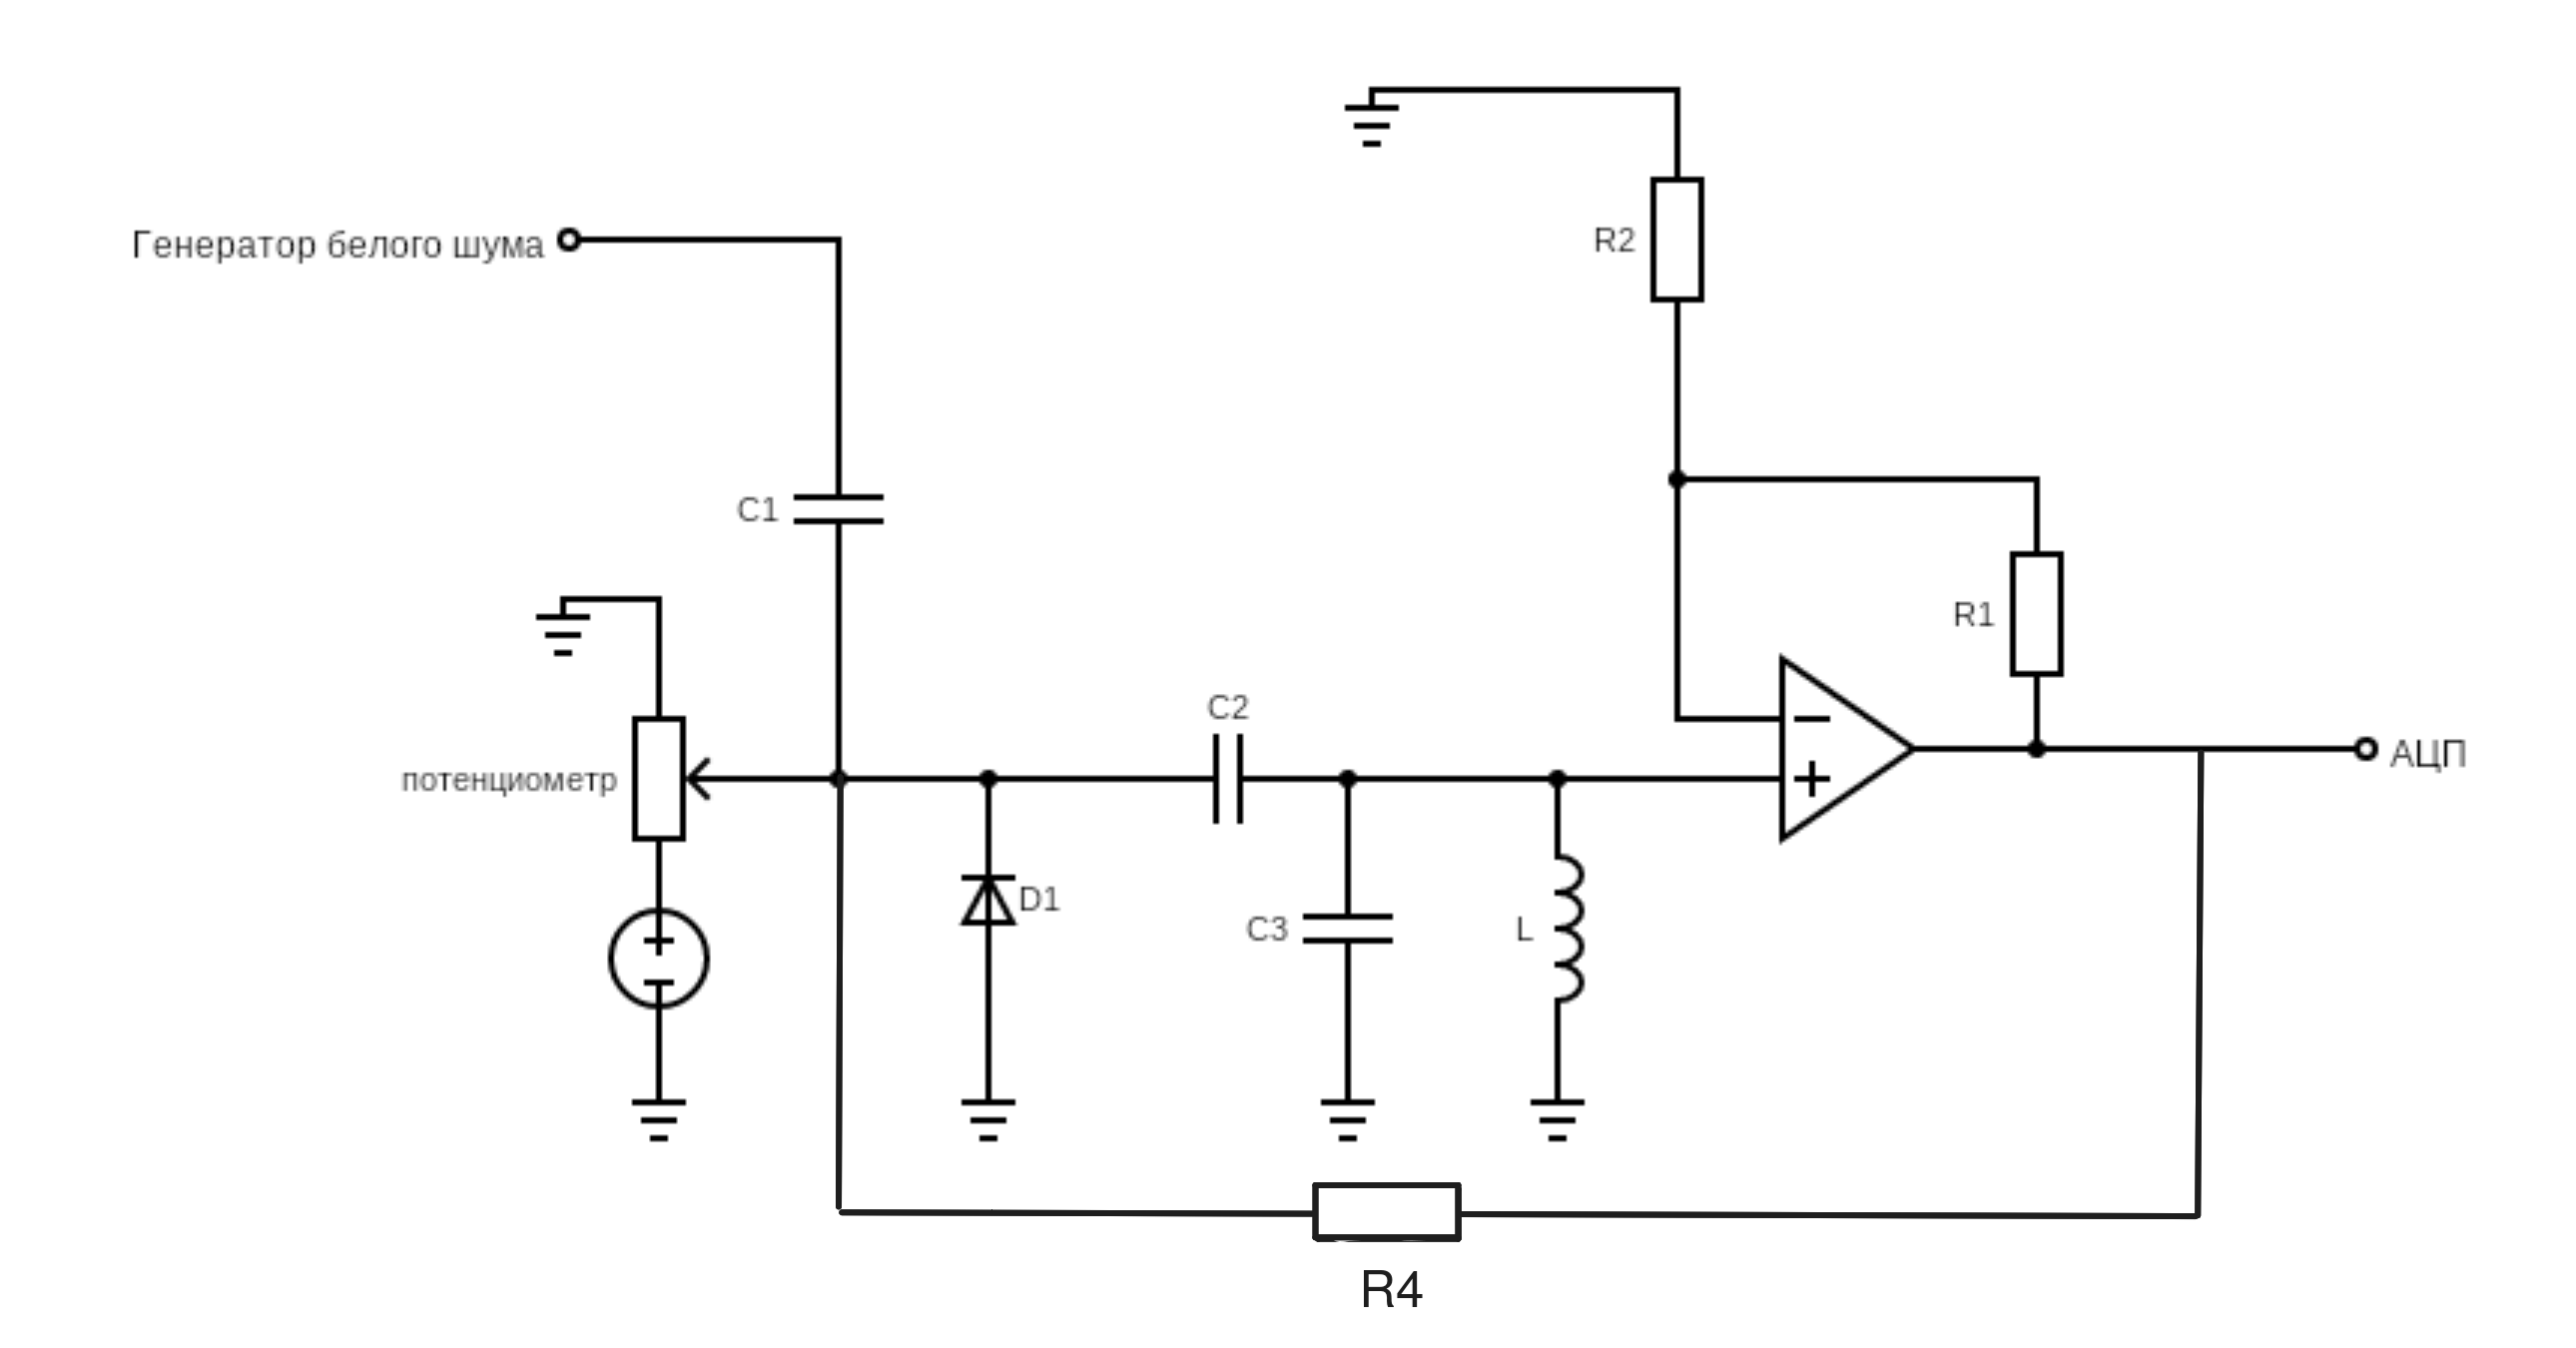
\includegraphics[width = 0.85\textwidth]{pics/main.png}
    \caption{Схема для измерения зависимости ёмкости диода от величины обратного напряжения.}
    \label{fig:main_scheme}
\end{figure}

Cхема экпериментальной установки представлена на рисунке $\ref{fig:main_scheme}$.
Напряжение на диоде D1 задаётся при помощи потенциомера. 
В качестве источника напряжения используется батарейка <<крона>>.
Конденсаторы C1 и C2 используются для отделения переменного сигнала(белого шума) от постоянного напряжения, 
задаваемого потенциометром.

Выходной сигнал усиливается при помощи ОУ, работающего в режиме неинвертирующего усилителя.
Для последующего анализа, усиленный сигнал оцифровывается.

Конденсатор C3, катушка L и диод D1 соединены параллельно и образуют LC контур. 
Меняя величину обратного напряжения на диоде, изменяется суммарная ёмкость. Изменение
ёмкости приводит к изменению частоты.
 

Конденсатор C3 имеет ёмкость $20 \mu F$ и был подобран экпериментально для получения резонансной
частоты в области звуковых частот. Резисторы R1 и R2 имеют сопротивления 4.7 кОм и 100 кОм соответсственно.
Таким образом, коэффициент усиления равен $K = 1 + 100 / 4.7 \sim 22$. 

Для повышения добротности и бОльшего усиления резонансной частоты используем обратную связь - 
соединяем выход схемы со входом через сопротивление R4 $\sim 220 \text{Ом}$.

\section*{\textcolor{header}{Обработка экспериментальных данных}}

Найдём индуктивность катушки. Для этого отключим диод от схемы, и запишем сигнал.
Разложив сигнал в ряд Фурье и найдя в нём частоту резонансной гармоники - рассчитаем 
индуктивность по формуле Томпсона. В результате <<калибровочного>> эксперимента получили индуктивность


\begin{figure}[htbp]
    \centering
    \includegraphics*[width = 1 \textwidth]{plots/0.png}
    \caption{Сигнал записанный при напряжении 0 Вольт. Резонасная частота 3889.86 Гц}
    \label{fig:zero_volt_specturm}
\end{figure}
В качестве диода D1 подключим 6 параллельно соединённых полупроводниковых диодов.
Вращая ручку потенциометра, пронаблюдаем изменение резонасной частоты.

\begin{figure}[htbp]
    \centering
    \includegraphics*[width = 1\textwidth]{plots/0.1.png}
    \caption{Сигнал записанный при напряжении 0.1 Вольт. Резонансная частота 3865.94 Гц}
    \label{<label>}
\end{figure}

Зная индуктивность катушки L, можем рассчитать ёмкость LC контура(см. формулу $\ref{sum_capacity}$).
\begin{equation}
    \label{sum_capacity}
    f = \frac{1}{2 \pi \sqrt{LC_{\text{сумм}}}} \to C_{\text{сумм}} = \frac{1}{4 \pi^2 L f^2}    
\end{equation}

Суммарная ёмкость складывается из ёмкости шести диодов и ёмкости конденсатора C3. Тогда:
\begin{equation}
    \label{diode_capacity}
    C_{\text{диод}} = \frac{C_{\text{сумм}} - C_{3}}{6}
\end{equation}

Построим график зависимости ёмкости диода от величины обратного напряжения(рисунок $\ref{fig:pn_main}$).
\begin{figure}[htbp]
    \centering
    \includegraphics*[width = 0.9 \textwidth]{plots/pn.png}
    \caption{Вольт - фарадная характеристика диода.}
    \label{fig:pn_main}
\end{figure}

Как видно на рисунке $\ref{fig:pn_main}$. Ёмкость диода при нулевом напряжении оказалась равной нулю.
Частоты колебний цепи без диода D1 и с диодом совпали.

При повышении напряжения, ёмкость резко увеличиватеся и остаётся постоянной до напряжения
$V \sim 1.75 \text{ Вольт}$. При последующем увиличении напряжения ёмкость начинает падать. 
Спад хорошо аппроксимируется формулой $\ref{capacity_by_volt}$:  $V_0 \sim 1.3 \text{ В}$,
$K \sim 39 \text{ пФ} \cdot \text{В}^{1/ 2}$

\section*{\textcolor{header}{Вывод}}

Удалось экспериментальной найти зависимость ёмкости диода от величины обратного напряжения.

Описанный в работе эффект может применяться для построения генраторов с возможностью модуляции частоты.
Для построения фильтров с возможностью изменения частоты среза при помощи вшенего сигнала.

Для описанных выше задач, был разработан специальный тип диодов. Варикап диоды обладают
большей ёмкостью и более предсказуемой вольт-фарадной характеристикой.





\end{document}
